Zgodnie z przedstawionymi własnościami materiałowymi obrazowanie z rozdzielczością przekraczającą klasyczne ograniczenie dyfrakcyjne przy pomocy metaliwiąże się z dużymi stratami natężenia światła w wyniku absorbcji. Zwiększenie współczynnika transmisji przez wielowarstwy zawierające metal możliwe jest dzięki wykorzystaniu efektu rezonansowego tunelowania \cite{scalora-transparentmetal}. Chociaż zastosowanie zaproponowane w cytowanej pracy nie było związane z obrazowaniem, to możliwość uzyskania współczynnika transmisji rzędu 70\% dla wielowarstwy zawierającej łącznie 40nm srebra otwiera możliwości wysokiej transmisji i wykorzystania materiałów o ujemnym $\varepsilon$. Schemat wielowarstwy przedstawia rysunek \ref{fig:mulschem}. W proponowanym podejściu obrazowanie nadrozdzielcze nie wynika wprost z zastosowania materiału o $\varepsilon = -1$, ale z efektywnych anizotropowych właściwości powstałęgo w ten sposób  metamateriału \cite{ramakrishna2003imaging}. Przy pomocy przybliżenia ośrodka efektywnego, szerzej omówionego w rozdziale \ref{subart:effmedium}, możemy dobierając grubości warstw do parametrów stosowanych materiałów uzyskać metamateriał o $\varepsilon_z \to \infty$ i $\varepsilon_x \to 0$.

Przykład materiałów z w opisany sposób można konstruować wielowarstwę charateryzującą się transmisją bezdyrakcyjną prezentują wykresy na rysnuknu \ref{fig:multiex}.




\begin{figure}[tb]
	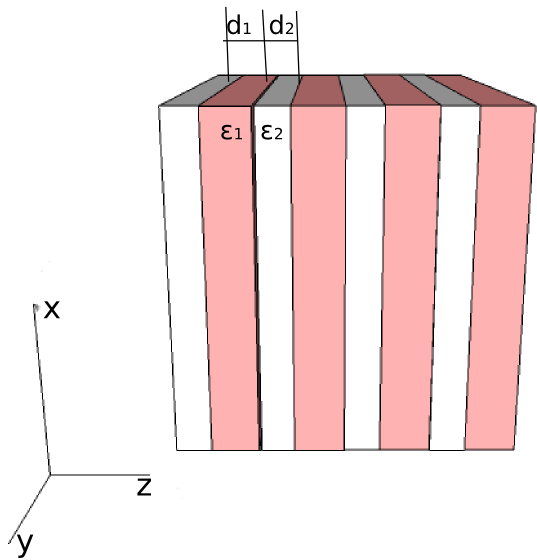
\includegraphics[width=.5\textwidth]{images/multilayer/multilayer-3d.png}
	\caption{Schemat wielowarstwy metaliczno dielektrycznej}
	\label{fig:mulschem}
\end{figure}

\begin{figure}[tb]
	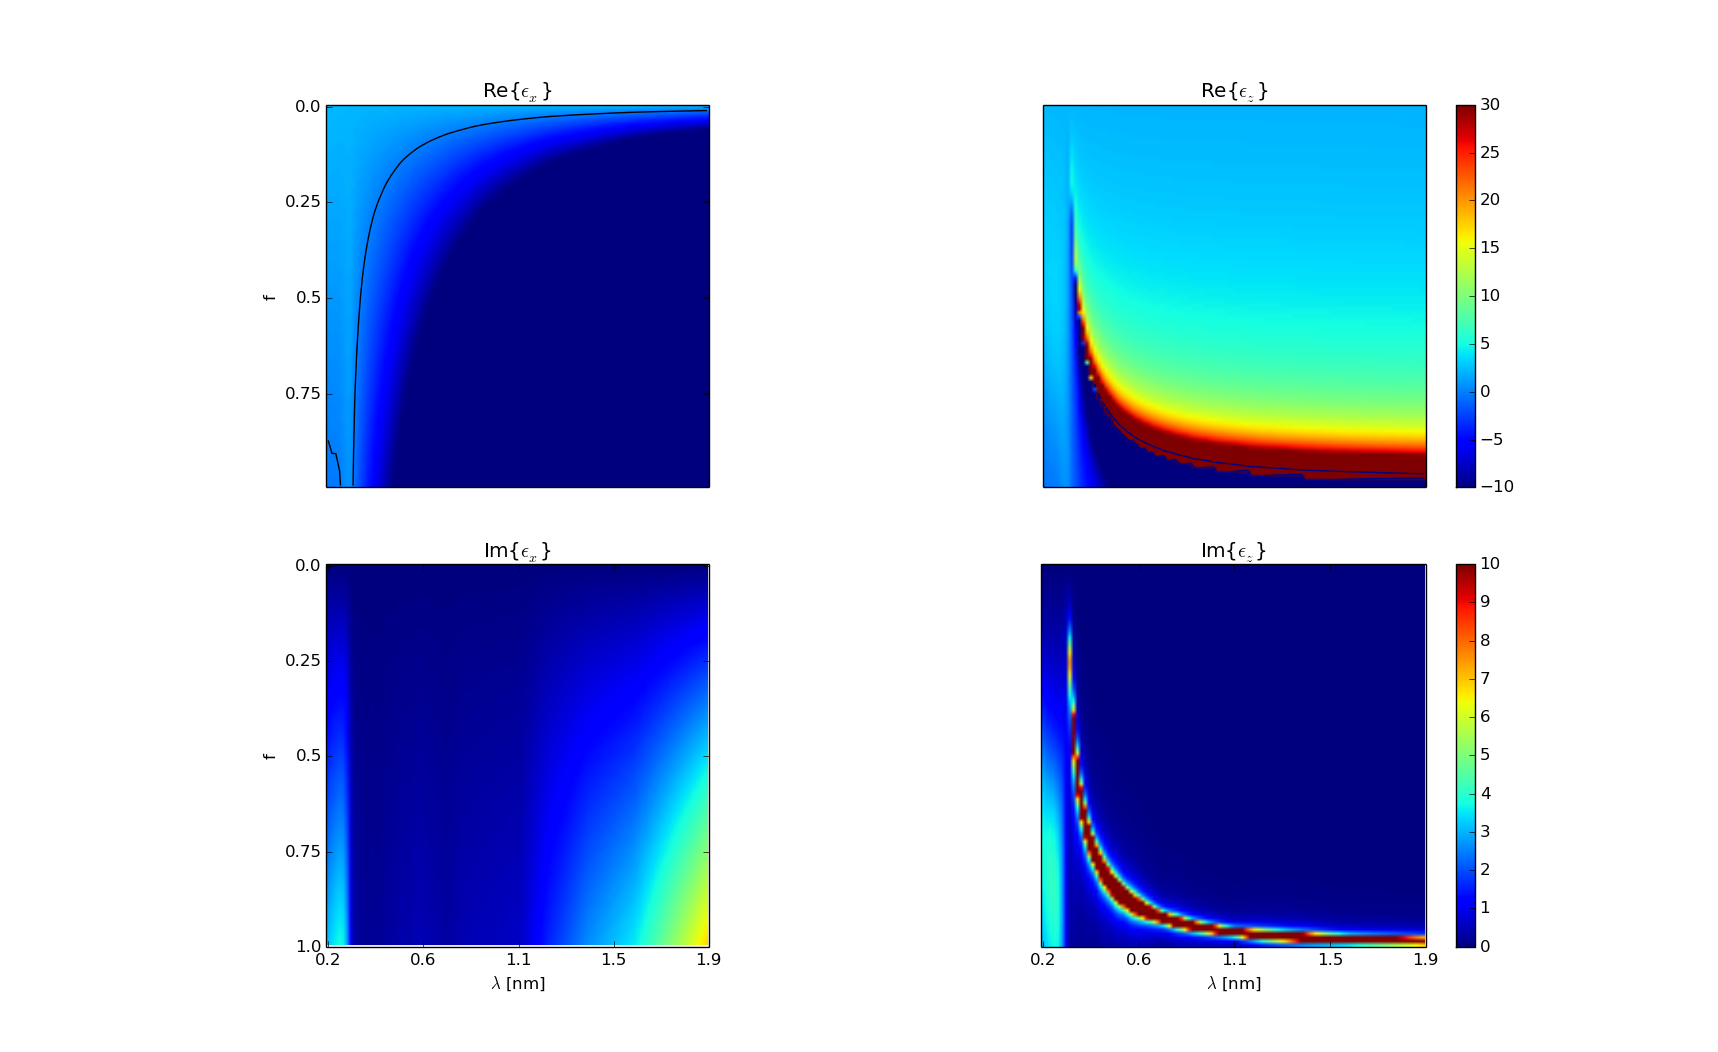
\includegraphics[width=1.5\textwidth]{images/multilayer/agsio2-effective.png}
	\label{fig:multiex}
	\caption{Przenikalność ośrodka efektywnego obliczona zgodnie z \ref{eq:effmedium}  zbudowanego z warstw $Ag$ \cite{PhysRevB.6.4370} i $SiO_2$ \cite{MALITSON:65}. Współczynnik wypełnienia f=1 oznacza, że struktura zbudowana jest jedynie ze srebra. Przy pomocy konturu zaznaczono $\varepsilon_x=0$ oraz $\varepsilon_z=100$.}
%generacja rysuknu:
%./effEpsilon.py database/main/Ag/Johnson.yml database/main/SiO2/Malitson.yml
\end{figure}

